\newpage
\thispagestyle{sectioned}
\chapter{Migración de Wave a Android}

\section{Estado del Arte}

 ---- PENDIENTE ----

\section{Wave}
  
  \subsection{Google Wave}

  Ideado y presentado en 2009 por ingenieros de Google \cite{ref:wave_announcement}, Wave es a la vez un protocolo de comunicaciones \cite{ref:wave_over_xmpp} y una plataforma web de código libre, que permiten a sus usuarios comunicarse y colaborar entre sí en tiempo real (Ver sección \ref{sssec:realTime}) y de forma federada (Ver sección \ref{sssec:federation}) a través de Internet. 
  Inicialmente fue desarrollado con el objetivo de integrar en una sola plataforma servicios ampliamente utilizados como son el correo electrónico, las redes sociales y la mensajería instantánea. Pese al gran entusiasmo generado entre la comunidad de desarrolladores tras su anuncio, en el año 2010 Google anuncia el abandono del proyecto \cite{ref:google_wave_end} debido a su poca acogida entre los desarrolladores y a que decide reorientar el uso de la tecnología hacia sus plataformas de edición de documentos Google Docs \cite{ref:google_docs} y a su red social Google + \cite{ref:google_plus}.  Es en este momento cuando el desarrollo libre del proyecto pasa a manos de la Apache Software Foundation bajo el nombre de Apache Wave.

  \subsection{Apache Wave}
  
  Al cambiar de manos su desarrollo en 2010, la tecnología pasa a formar parte de la incubadora de la fundación Apache \cite{ref:apache_wave_about} como software de código libre bajo licencia Apache \cite{ref:apache_license}. Así, se produce el desarrollo de Wave In a Box (WIAB) (Ver sección \ref{sec:wiab}), plataforma que integra un cliente web sencillo y una implementación de un servidor Wave que cualquiera puede descargar y desplegar en su ordenador.   

\section{Tecnologias y Caracteristicas de Wave}
  
  \subsection{Caracteristicas de Wave}
  
  Como plataforma de código libre desarrollada para ser utilizada en red, Wave hace uso de distintas tecnologías y protocolos bien conocidos. Entre sus características más destacadas están las siguientes:

    \subsubsection{Federación}\label{sssec:federation}
    
    El Protocolo Wave \cite{ref:wave_over_xmpp} fue desarrollado para utilizar un modelo federado \cite{ref:wave_federation} \cite{ref:wave_white_paper} de comunicación basado en la tecnología XMPP \cite{ref:xmpp} \cite{ref:wave_over_xmpp}. Se trata por tanto de un modelo descentralizado en el que cualquiera de los participantes en la conversación es libre de actuar tanto como servidor como cliente sin que ello afecte a su participación en la conversación. 
    Además, a diferencia de otras tecnologías (como el correo electronico) en las que cada participante almacena su propia copia de la conversación y cada vez que hay cambios se debe transmitir la conversación entera a todos los participantes, Wave tiene la ventaja de que actúa de forma que es el servidor de la conversación el único que almacena la copia entera y se encarga de calcular los cambios que se han producido para transmitir solamente dichos cambios por la red a los participantes, con las consiguientes ventajas en términos de latencia que ello conlleva. 

    \subsubsection{Consistencia en tiempo real}\label{sssec:realTime}
    
    El Protocolo Wave \cite{ref:wave_over_xmpp} utiliza la tecnología de Transformaciones Operacionales (OT) \cite{ref:how_ot_works} para garantizar la consistencia en la comunicación en tiempo real entre los participantes. Es decir, cualquier cambio producido por cualquiera de los participantes en la conversación se transmite automáticamente y en tiempo real al resto de los participantes sin pérdida de información y garantizando que los cambios se muestran en el estricto orden en el que se produjeron sin errores \cite{ref:wave_ot}.
    
    \subsubsection{Escalabilidad}
    
    Wave fue desarrollado como un protocolo de alta escalabilidad que permite gestionar la existencia de una gran cantidad de conversaciones y participantes sin que por ello se resienta la productividad del sistema.
    
    \subsubsection{Modelo Wave}\label{sec:waveModel}
    
    Además de definir el protocolo del que hace uso Wave, Google definió un Modelo de Datos Conversacional \cite{ref:wave_conversation_model} que refleja la arquitectura de los datos que componen las conversaciones en Wave. Así, a grandes rasgos, podemos ver dichas conversaciones como documentos XML sobre los que los usuarios participantes (cualquiera es libre de unirse a una conversación en cualquier momento) actúan creando nuevos elementos o modificando los ya existentes. Este modelo de datos define una nomenclatura propia para los elementos que componen esta tecnología \cite{ref:wave_api_overview} \cite{ref:wave_white_paper}:
    
      \begin{itemize}
	\item \textbf{Wave}: Conjunto de wavelets (conversaciones).
	\item \textbf{Wavelet}: conjunto de documentos de una conversación y sus participantes.
	\item \textbf{Blip}: documento con el contenido de un mensaje en la conversación. Un blip puede tener otros blips dentro de él y los blips pueden ser publicados o no en función de si su visibilidad se extiende o no al resto de participantes de la conversación respectivamente.
	\item \textbf{Manifiesto conversacional}: documento con metadatos que definen la estructura de una conversación. 
	\item \textbf{Hilo conversacional}: conjunto de Blips consecutivos que forman parte de una conversación.
	\item \textbf{Extensiones} \cite{ref:wave_extensions}: pequeñas aplicaciones que se ejecutan dentro de una Wave y aportan nuevas funcionalidades que no forman parte del modelo conversacional básico. Pueden ser de dos tipos:
	  \begin{itemize}
	    \item \textbf{Gadget}: aplicación que se ejecuta en el contexto de una Wave y en la que todos sus usuarios participan.
	    \item \textbf{Robot}: aplicación que participa en una Wave a modo de usuario automatizado e interactúa con el contenido pudiendo modificarlo y responder a eventos por acciones de otros usuarios reales.
	  \end{itemize}
      \end{itemize}
      
       \begin{figure}[H]
	  \centering
	    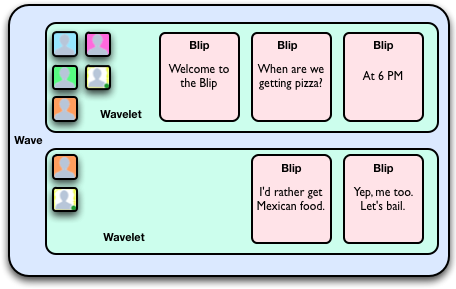
\includegraphics[keepaspectratio, scale=0.8]{Media/Captures/waveEntities.png}
	  \caption{Modelo Conversacional de Wave}
	  \label{fig:wave_model}
	\end{figure}
  
  \subsection{Servidores Wave}
  
    \subsubsection{Wave in a Box}\label{sssec:wiab}
    
    Wave In a Box (WIAB) \cite{ref:wave_in_a_box} es el nombre de la implementación de un servidor Wave desarrollado por la Apache Software Foundation tras pasar el proyecto a sus manos en el año 2012. Al igual que el resto del código de la tecnología que heredó de Google, está implementado en Java usando OpenJDK \cite{ref:openjdk}. La instalación trae consigo un cliente web desarrollado en Javascript usando el framework Google Web Toolkit \cite{ref:gwt}. Este cliente web sirve como prueba de concepto de las funcionalidades básicas del Modelo Conversacional de Wave, pudiendo gesionar waves, usuarios y extesiones. Actualmente cualquiera puede descargar y desplegar WIAB en su ordenador siguiendo los pasos que nos proporcionan en su wiki \cite{ref:wave_in_a_box_wiki}. La aplicación se distribuye en forma de código fuente, accesible entre otras formas desde su repositorio de GitHub \cite{ref:wave_in_a_box_github}. Existen asimismo servidores de prueba ya desplegados en Internet sobre los que se puede observar el funcionamiento de WIAB \cite{ref:wave_in_a_box_server}.
   
   
    \begin{figure}[H]
      \centering
	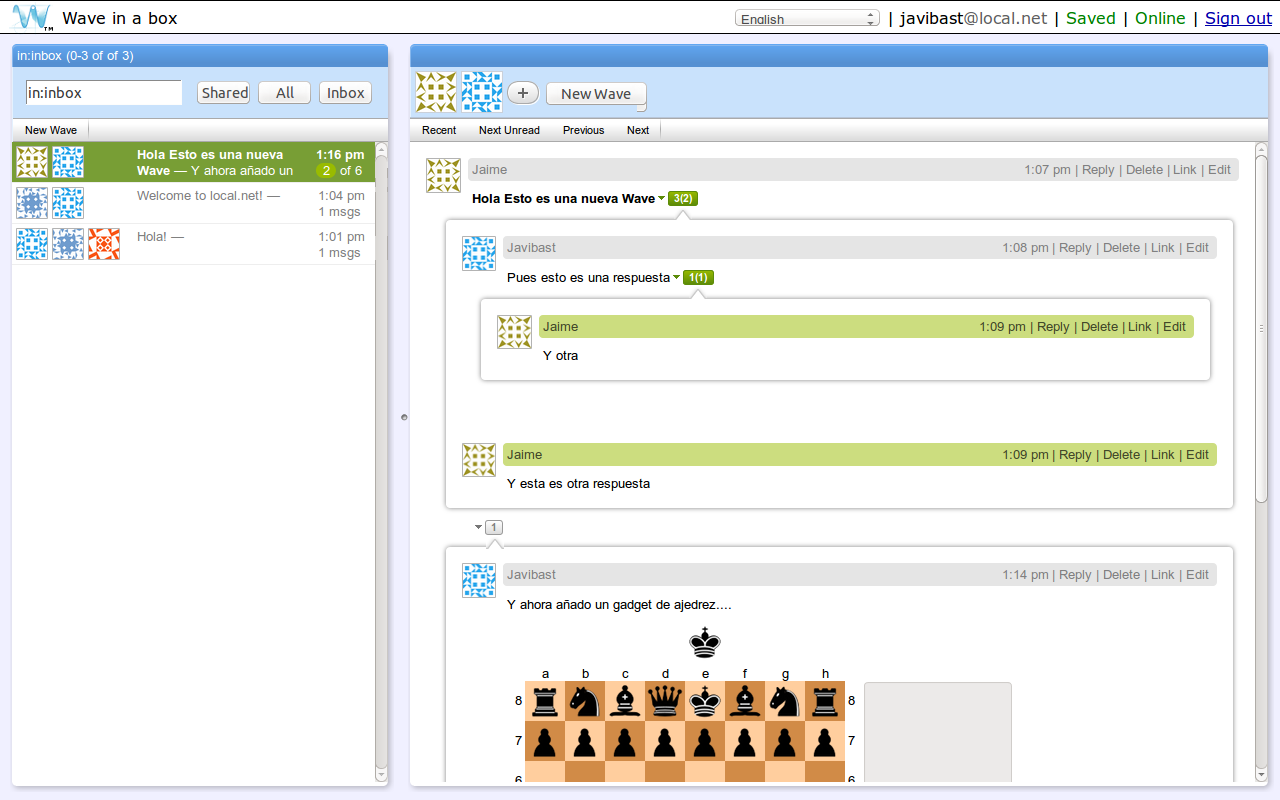
\includegraphics[keepaspectratio, scale=0.3]{Media/Captures/WIAB_Server.png}
      \caption{Cliente Wave In A Box}
      \label{fig:wiab_client}
    \end{figure}
   
    \subsubsection{SwellRT}\label{sssec:swellRT}
    
    Como parte del proyecto europeo P2PValue \cite{ref:p2pvalue} existe SwellRT, un fork de WIAB que amplía las características de éste último añadiendo un nuevo modelo de datos (Modelo de Datos Colaborativo) más allá del Modelo de Datos Conversacional de Wave original. Proporciona también un API escrito en Java que permite trabajar sobre los datos de ese nuevo modelo en forma de tres tipos básicos: mapas, listas y strings. Es por tanto un framework de colaboración en tiempo real que basa su funcionamiento en Apache Wave y cuyo principal popósito es permitir la integracion de la tecnología Wave en otras aplicaciones, que podrán compartir objetos (de los tipos antes mencionados) de forma federada y en tiempo real. Su código fuente está disponible en GitHub \cite{ref:swellRT_github}, así como sus instrucciones de instalación (Ver el Readme en GitHub).\\[.2cm]

    Para este proyecto se ha usado el framework SwellRT como base para la migración de la tecnología de Apache Wave a la plataforma Android \cite{ref:android_platform}. Se pretende con esto que SwellRT haga uso de las funcionalidades nativas de Android.

  
\section{Metodología de Migración}
  
  \subsection{Objetivo}
  
    El framework de SwellRT utiliza un servidor WIAB y el protocolo Wave, ambos desarrollados en Java. El \textbf{SDK de Android} \cite{ref:android_sdk} es compatible con Java, así que a priori la implantación del servidor no supone problemas en los dispositivos móviles. Sin embargo, existe un problema con el API de SwellRT, ya que el lado del cliente fue desarrollado en Javascript usando el framework GWT. Android no soporta de forma nativa estas tecnologías, así que es necesario estudiar el código de SwellRT para sustituir todo el código que haga uso de Javascript/GWT por código compatible con Android. El objetivo de esta parte del proyecto es conseguir que un cliente desplegado en Android sea capaz de conectarse e interactuar con un servidor Wave sin problemas.  
  
  \subsection{Plataforma: Entorno de Desarrollo, Construcción y Depuración}
  
    Existen dos entornos de desarrollo (IDE) recomendados por Google para desarrollar en Android: Eclipse \cite{ref:eclipse} y Android Studio.\cite{ref:android_studio} Eclipse es un entorno de desarrollo genérico que, mediante plugins, permite extender sus funcionalidades para desarrollar en diversas plataformas y lenguajes. Android Studio es un IDE basado en el entorno de desarrollo Java IntelliJ IDEA \cite{ref:intelliJ_Idea} adaptado para trabajar con todas las funcionalidades de Android. En el momento de empezar con la migración Android Studio se encuentra en fase beta de desarrollo, pues Google pretende convertirla en el IDE de desarrollo oficial para Android. Mientras no se lanza la version final de Android Studio, Google recomienda utilizar Eclipse para desarrollar en Android, y las guias para desarrolladores Android estan escritas para Eclipse. En consecuencia tomamos la decision de utilizar el entorno de desarrollo Eclipse para la migracion de SwellRT a Android. 

    \subsubsection{Eclipse} \label{sssec:eclipse}
    
    El IDE de Eclipse \cite{ref:eclipse} soporta el desarrollo con Android a través del plugin \textbf{ADT (Android Development Tools)} \cite{ref:eclipse_adt}, que integra en un solo paquete todas las herramientas necesarias para desarrollar, construir y depurar el código de la aplicacion fácilmente. \\[.2cm]
    
    \textbf{Android SDK} \cite{ref:android_sdk}: paquete que integra el conjunto de herramientas necesarias para desarrollar en Android.  Entre estas herramientas destacan las siguientes:
    
    \begin{itemize}
    \item \textbf{Librerías con el API} de Android y \textbf{Documentación} asociada \cite{ref:android_api_reference}
    
    \item \textbf{Android Virtual Device Manager (AVDM)} \cite{ref:android_vdm} herramienta para gestionar la creación, modificación, ejecución y eliminación de emuladores en Android. Un \textbf{emulador} \cite{ref:android_emulator} es una máquina virtual que ejecuta una determinada versión de Android. Permite desplegar un dispositivo movil en el ordenador que imita las características software y hardware de uno real para poder hacer pruebas de desarrollo sin necesidad de poseer un dispositivo con Android. 
    
    \item \textbf{Android SDK Manager} \cite{ref:android_sdk_manager} herramienta para gestionar las versiones de SDK y herramientas asociadas instaladas. Android se encuentra actualmente en la versión 5.1 (API 22), pero un desarrollador puede elegir desarrollar para una versión anterior si lo estima necesario, por lo que puede descargarse por separado dicha versión y mantener varias API si lo necesita.
    
    \item \textbf{Dalvik Debug Monitor Server (DDMS)} \cite{ref:android_ddms} herramienta que provee las características de entorno de depuración para las aplicaciones en desarrollo.

    \end{itemize}
	
	Teniendo en cuenta la distribucion actual de versiones instaladas en dispositivos Android \cite{ref:android_dist} (Ver figura \ref{fig:android_Usage}) se ha decidido realizar la migración de SwellRT con el API 19 de Android (Version 4.4 "KitKat"). El emulador desplegado para las pruebas de desarrollo utilizará por tanto Android 4.4 .

	\begin{figure}[H]
      \centering
	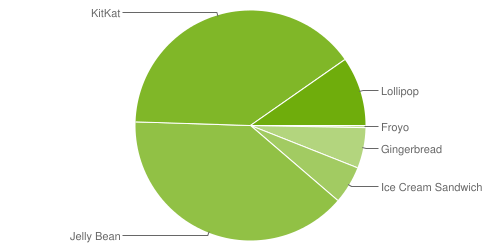
\includegraphics[keepaspectratio, scale=0.8]{Media/Captures/androidUsage.png}
      \caption{Distribución Actual de Versiones Android (Fuente: Google)}
      \label{fig:android_Usage}
    \end{figure}

	Sin embargo existe un problema con la construcción y depuración del código de SwellRT en Eclipse. Android \textbf{limita el número de métodos máximos de una aplicacion a 65K} \cite{ref:android_limit65k} por cuestiones de eficiencia. Para evitar esta limitación, durante el proceso de construcción el SDK de Android utiliza, entre otras, una herramienta llamada \textbf{ProGuard} \cite{ref:android_proguard}. Esta herramienta se encarga de optimizar el código de la aplicacion buscando remover clases que no se utilizan y ofuscando el código para prevenir la ingeniería inversa. En el caso de SwellRT, el código posee un gran número de clases java necesarias para desplegar el servidor y el cliente de la herramienta, por lo que es necesaria dicha optimización de código realizada por ProGuard. El sistema de compilación de aplicaciones de Android tiene dos formas: compilacion de la aplicacion en modo debug (para hacer pruebas cuando todavía se encuentra en fase de desarrollo) y en modo release (la aplicación se encuentra en su versión final y se empaqueta y se firma digitalmente para lanzarla al público). En el caso de Eclipse, ProGuard solo se ejecuta cuando se construye en modo release, por lo que cuando se intenta compilar una aplicación con tantas clases como SwellRT mientras se desarrolla (modo debug) el sistema da error y no se puede compilar el código para probarlo en el emulador. \\[.2cm]

	La solución que encontramos fue desarrollar en Eclipse (por las facilidades que el entorno proporciona para escribir código) pero realizar el proceso de construcción del código por consola de comandos, ya que en este caso sí que se puede compilar la aplicación en modo debug utilizando ProGuard.

	     
    \subsubsection{Proceso de Construcción por Consola}

		Para construir la aplicación por consola de comandos, Android utiliza la herramienta Apache Ant \cite{ref:ant} para automatizar el proceso de construcción \cite{ref:android_cmd_line}. Es importante asimismo tener definida la variable de entorno JAVA\_HOME con la ruta de acceso al JDK de java instalado en la máquina. Conviene también, por comodidad a la hora de trabajar con la consola, añadir al PATH del sistema las rutas a la carpeta donde esta el SDK de android (/sdk) y dentro de esta ruta añadir asimismo rutas a las carpetas /tools y /platform-tools. \\[.2cm]

Existen dos formas de realizar la construcción en modo debug de una app: \\[.2cm] 

\textbf{1 - Sin tener previamente lanzado un emulador o conectado al ordenador un dispositivo android en modo debug \cite{ref:android_device_setUp}:} \\[.2cm]
 
 	 En este caso es necesario construir la aplicación y luego lanzar el emulador para después instalar la aplicación en él. Para construir la aplicacion en modo debug nos vamos a la carpeta raíz de nuestro proyecto y ejecutamos el siguiente comando: 

 	 \begin{lstlisting}[style=console, numbers=none]
		$ ant clean debug
	 \end{lstlisting}
 	 
 	 Esto nos generará una aplicacion instalable en el directorio /bin del proyecto bajo el formato que Android usa para sus aplicaciones (.apk). El siguiente paso es ejecutar un emulador o conectar un dispositivo android por USB. Para ejecutar un emulador, abrimos otra consola y utilizamos el siguiente comando:
 	 
 	 \begin{lstlisting}[style=console, numbers=none]
		$ android avd
	 \end{lstlisting}
 	 
 	 Lo que nos despliega la herramienta Android Virtual Device Manager (Ver Seccion \ref{sssec:eclipse}) para que elijamos/creemos el emulador que queremos ejecutar. Podemos elegir multitud de parámetros \cite{ref_android_avd_params} para el dispositivo que emula (resolución y tamaño de pantalla, de memoria Ram, elementos hardware emulados, etc.) siendo lo más importante elegir un API (versión de Android) que se corresponda con el API que hemos elegido para nuestra aplicación (en nuestro caso API 19). Es recomendable también elegir una imagen del sistema que use un procesador con arquitectura Intel x86, ya que si elegimos la opción por defecto de ARM (los dispositivos móviles actuales usan procesadores ARM) la ejecución del emulador se ralentiza mucho al tener que emular una arquitectura de procesador distinta a la suya (los ordenadores actuales usan arquitectura Intel x86 en su mayoría). Esto únicamente afecta al rendimiento del emulador, la aplicación es independiente de la arquitectura que haya por debajo. \\[.2cm]
 
     Una vez lanzado el emulador/dispositivo móvil, procedemos a instalar la aplicación en él ejecutando el siguiente comando en la primera consola (en la que construimos la aplicacion):
		      	 
 	 \begin{lstlisting}[style=console, numbers=none]
		$ adb install XXXX.apk
	 \end{lstlisting}		
 	 
 	 Siendo XXXX la ruta a donde se encuentra el .apk de la aplicación que previamente hemos construido (/bin). La herramienta ADB (Android Debug Bridge) \cite{ref:android_adb} es la que permite la comunicación entre el proceso de la consola de comandos y el emulador/dispositivo móvil. Es importante destacar que si se tienen varios emuladores/dispositivos moviles en ejecucion/conectados hay que especificar en cual se quiere instalar la aplicación añadiendo al comando lo siguiente: \textbf{-s emulator -YYYY} siendo esto último el identificador del emulador que podemos encontrar en el título de la ventana del emulador. \\[.2cm]
	     
	\begin{figure}[H]
      \centering
	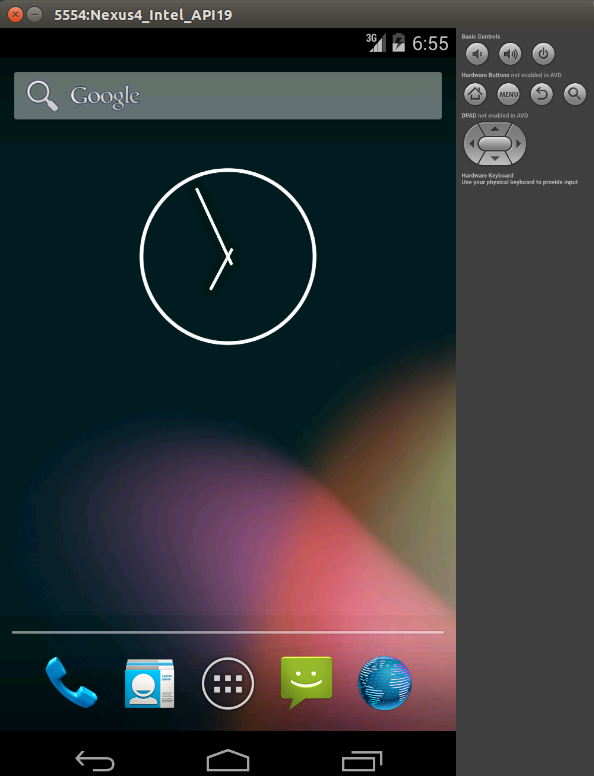
\includegraphics[keepaspectratio, scale=0.3]{Media/Captures/emulator_api_19.png}
      \caption{Emulador Android API 19}
      \label{fig:android_emulator19}
    \end{figure} 
    
    De esta manera podemos probar la aplicación, que será lanzada en el emulador/dispositivo una vez termine su instalación. \\[.2cm]

	\textbf{2 - Teniendo un emulador previamente lanzado (ver sección anterior para ver cómo se lanza) o un dispositivo móvil ya conectado por USB:} \\[.2cm]
	
	En este caso es todavía más sencillo el proceso de construcción. Nos vamos a la carpeta raíz del proyecto  y podemos compilar e instalar la aplicación con un solo comando:

 	 \begin{lstlisting}[style=console, numbers=none]
		$ ant debug install
	\end{lstlisting}	
 	 
 	 Es importante destacar que este comando solo funciona si tenemos un único emulador o dispositivo conectado, de lo contrario habrá que utilizar el método anterior. \\[.2cm]

    
    \subsubsection{Proceso de Depuración} \label{sssec:debug}
    
    Una vez instalada una aplicación, podemos depurar su código en ejecución usando la herramienta DDMS del ADT en conjunto con la vista de Debug de Eclipse. Pero antes hay que especificar qué aplicación queremos depurar de las que puedan estar instaladas en el dispositivo o emulador. \\[.2cm]

En el caso del emulador debemos lanzar la aplicación llamada “Dev Tools” y abrir el menú “Developer Options”. Dentro de este menú habilitaremos las opciones de “USB debugging” y de  “Wait for debugger”. Además pulsaremos sobre “Select Debug app” y seleccionaremos la aplicación que queremos depurar. \\[.2cm]

En el caso de un dispositivo Android debemos ir a los Ajustes del dispositivo y seleccionar el menú de Opciones de Desarrollador. Aquí habilitamos las opciones de "Depuración de USB"  (si no esta habilitada ya) y de "Esperar al depurador". Además pulsamos donde pone "Seleccione una aplicación para depurar" y elegimos la aplicación que queremos depurar. \\[.2cm]

Una vez hecho esto, cada vez que ejecutemos la aplicacion saldrá un mensaje de advertencia y se quedará esperando a que conectemos un depurador para continuar con su ejecución. Para esto, nos vamos a Eclipse y abrimos la vista de DDMS. Aquí nos aparecerá, entre otras cosas, un espacio con todos los procesos en ejecución en el dispositivo/emulador. Localizamos el proceso de nuestra aplicación y pulsamos sobre el bichillo verde para conectar el depurador a ella. Llegados a este punto la aplicacion continua su ejecución en el emulador y aparece un escarabajo verde al lado del proceso de la app en la ventana de DDMS, que indica que se esta depurando ese proceso. Es entonces cuando podemos abrir la vista de depuración de Eclipse y proceder a trabajar con breakpoints para depurar y estudiar el código con el fin de solucionar errores.

    
  \subsection{Migración: Identificación y Solución de Problemas}
  
	  El objetivo de esta parte del proyecto es conseguir que el cliente de SwellRT se pueda desplegar en Android para asi conseguir que se conecte al servidor WIAB que tambien incluye. Para ello lo primero que haremos será desplegar el servidor en nuestro ordenador clonando el repositorio de GitHub de SwellRT y siguiendo los pasos descritos en el Readme del proyecto \cite{ref:swellRT_github}. Para comprobar que el servidor se ha instalado correctamente, podemos ejecutarlo por consola (ver Readme) y abrir un navegador web con la dirección http://localhost:9898. Si nos aparece una ventana de Login de WIAB es que ya tenemos un servidor WIAB corriendo en nuestro ordenador. Creamos entonces un usuario y contraseña de prueba. Este paso es importante ya que la aplicación Android intentará conectarse contra este servidor mientras estemos haciendo pruebas de desarrollo. \\[.2cm]
	  
	  A continuación crearemos un proyecto Android en Eclipse e incluiremos en él todas las clases de SwellRT. Uno de los componentes principales de Android a la hora de desarrollar son las \textbf{Actividades} \cite{ref:android_activities}, que representan las pantallas que se le muestran al usuario y que responden a su interacción programáticamente. Por tanto, crearemos una nueva actividad  
	  principal (waveAndroid.java) que se ejecutará al lanzar la aplicación y que por el momento intentará conectarse al servidor especificando por código el usuario y contraseña que hemos creado antes en el servidor. Wave realiza este login contra el servidor usando dos tecnologias: HTTP \cite{ref:http_authentication} y WebSockets \cite{ref:webSocket_ref}.
	  
  
    \subsubsection{Conexion HTTP}\label{sssec:conHttp}
	
	Wave fue desarrollado para utilizar el protocolo WebSocket para la conexión al servidor, pero esta tecnología necesita realizar una autenticación HTTP previa. Lo primero que haremos será otorgar \textbf{permisos de conexión a internet} a nuestra aplicación. Android utiliza un \textbf{sistema de permisos} \cite{ref:android_permissions} para controlar los privilegios de cada aplicación. Estos permisos se declaran en el \textbf{Manifiesto} de la aplicación \cite{ref:android_manifest}, archivo que declara sus características. Para ello basta con añadir lo siguiente al manifest.xml de la aplicación:
	  
	  \lstset{language=XML, breaklines=true, autogobble=true, basicstyle=\ttfamily\footnotesize}
	  \begin{lstlisting}[frame=single]
	  	<uses-permission android:name="android.permission.INTERNET"/>
	  \end{lstlisting}
	  
	  	 Tambien hay que tener en cuenta que cuando nos encontramos en el emulador no estamos en la misma red que el ordenador en el que trabajamos, por lo que la conexion a la URL http://localhost:9898 no es valida. No obstante, esto tiene facil solucion pues \textbf{el emulador de Android define unas direcciones IP de red especiales} \cite{ref:android_netAddress} para este tipo de casos. Basta con sustituir localhost por la direccion 10.0.2.2 para conseguir acceder al servidor WIAB desplegado en el ordenador. La direccion URL sera por tanto: \textbf{http://10.0.2.2:9898}. 
	  
	 Lo siguiente que haremos será ejecutar el código de Login del cliente SwellRT para intentar localizar dónde se lleva a cabo la conexion HTTP. Para ello llamamos desde la actividad principal (WaveAndroid.java) al método startSession() de la clase WaveClient.java pasándole el usuario y la contraseña antes creados.
 
	 Esto provoca un error de ejecución y la aplicación se cierra. Lo siguiente que hacemos es depurar la aplicación (Ver Seccion \ref{sssec:debug}) estudiando el LogCat \cite{ref:android_logcat} (Ver Figura \ref{fig:android_logcat}) para ver donde se produce el error. Descubrimos que el problema estaba localizado en el método login() de la misma clase, que intentaba realizar una \textbf{peticion POST HTTP} al servidor utilizando un \textbf{RequestBuilder} de la libreria \textbf{com.google.gwt.http.client}. He aquí el primer problema: la actual conexión utiliza métodos de GWT/Javascript para hacer la petición post y Android no es compatible con esta tecnología.   
	 
	\begin{figure}[H]
      \centering
	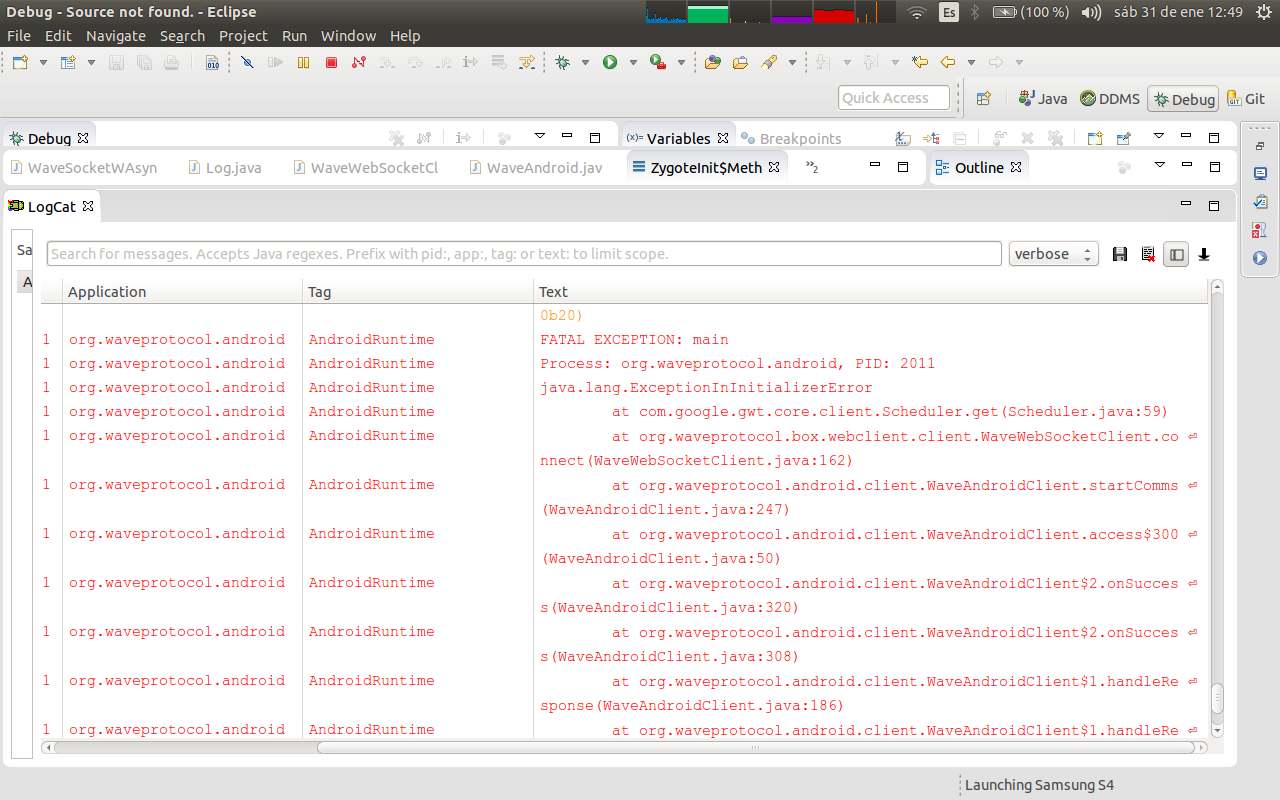
\includegraphics[keepaspectratio, scale=0.3]{Media/Captures/logcat_example.png}
      \caption{Ejemplo de Traza de Error en Logcat}
      \label{fig:android_logcat}
    \end{figure} 
	 
	 Hay por tanto que encontrar una librería similar compatible con Android que construya una peticion \textbf{HTTP POST} y la envie al servidor. La primera opcion que valoramos fue utilizar la \textbf{libreria HTTP Apache} \cite{ref:apache_http}, incluida en el SDK de Android desde sus primeras versiones. Sin embargo, Google recomienda \cite{ref:http_recommmendations} a partir del API 10 (Android 2.3 "Gingerbread") utilizar la \textbf{libreria HttpURLConnection} \cite{ref:android_httpUrlConnection}. Por tanto esta ultima es la que elegimos para la migracion. \\[.2cm] 
	 
	 De forma simplificada, este seria un esquema de la nueva estructura del login HTTP:
	 
	  \lstset{language=Java, breaklines=true, autogobble=true, basicstyle=\ttfamily\footnotesize, commentstyle=\color{OliveGreen}, keywordstyle=\color{MidnightBlue}}
	  \begin{lstlisting}[frame=single]	  
import java.net.HttpURLConnection;

private void login(final String user, final String password, final Callback<String, String> callback) {
  
		//Construct the URL String urlStr with the server, user and password parameters
  
	    URL url = new URL(urlStr); //String 
	    HttpURLConnection connection = (HttpURLConnection) url.openConnection(); //Open the connection to the given URL

	    connection.setDoOutput(true); // allow the POST connection
	    connection.setRequestProperty("Accept-Charset", CHARSET);
	    connection.setRequestProperty("Content-Type", "application/x-www-form-urlencoded;charset="
		+ CHARSET);

	    OutputStream out = connection.getOutputStream(); 
	    out.write(queryStr.getBytes(CHARSET)); //Set the POST parameters

	    if (connection.getResponseCode() != 200) {
		      //ERROR during the connection
		      connection.disconnect(); //Disconnect from the server.
	    } else {
		      //Continue with the login process (WebSocket)
		      connection.disconnect(); //Disconnect from the server.
	    }		      
}	    
	  \end{lstlisting}  
	  
	  Sin embargo, aquí no acaba el problema. Por cuestiones de usabilidad y de respuesta a la interacción del usuario, Android establece dos reglas para trabajar con el proceso de la actividad que se le esta mostrando al usuario (llamado \textbf{UI Thread}) \cite{ref:android_processes}:
	  
	  \begin{itemize}
	  	\item \textbf{1. No bloquear el UI Thread}
	  	\item \textbf{2. No acceder al UI Thread directamente desde otro Thread}
	  \end{itemize}
	  
	  La conexión a un servidor es un proceso susceptible de durar un tiempo variable según las condiciones de la red, lo cual deja la aplicación en espera hasta que se realiza dicha conexión,  bloqueando el UI Thread. Por tanto, decidimos usar un hilo (Thread) por separado en forma de \textbf{AsyncTask} \cite{ref:android:asynctask} para llevar a cabo la tarea de Login, tal y como recomienda Google hacer para trabajar con conexiones a la red \cite{ref:android_networking}. La ventaja por tanto de usar otro hilo para esto es que la actividad principal no se bloquea. \\[.2cm]
	  	 
	  El siguiente es un esquema del AsyncTask encargado del Login: \\[.2cm]
	  
	  \lstset{language=Java, breaklines=true, autogobble=true, basicstyle=\ttfamily\footnotesize, commentstyle=\color{OliveGreen}, keywordstyle=\color{MidnightBlue}}
	  \begin{lstlisting}[frame=single]	  
private class LoginTask extends AsyncTask<String, Void, String> {

    @Override
    protected String doInBackground(String... params) { //method that executes on the new Thread without blocking the UI Thread
      login(params[0], params[1], params[2]); //Do the login     
    }

    @Override
    protected void onPostExecute(String result) { //method that executes on the UI Thread once doInBackground() finishes its execution.
    
      if (result != null) { 
        callback.onLogin(); //Notify the login success using the proper callback method
      } else { //The doInBackGround method has had a problem and the result of its execution was null
        callback.onError("Wave Login Error"); //Notify the login error using the proper callback method
      }
    }
}    
	  \end{lstlisting} 
	  
	  Es importante tambien destacar que la arquitectura de SwellRT y de Wave esta planteada de manera que utiliza llamadas asíncronas (callbacks) para notificar al resto de la aplicacion del resultado de los procesos de conexión al servidor.
	    
\textbf{Llegados a este punto, tenemos un proceso de login Http que hace uso de la libreria HttpUrlConnection y de un AsyncTask para realizar esa primera conexión al servidor.} Depuramos la aplicación y comprobamos que efectivamente el login Http se realiza correctamente (la respuesta del servidor tiene código 200). \textbf{Sin embargo la aplicacion aun no funciona correctamente, pues se cierra al intentar ejecutar el código que se encarga del siguiente paso del login: la conexión por WebSocket.}    
    
    \subsubsection{Conexión WebSocket}\label{sssec:conWave}
    
    Para realizar una conexión con el servidor Wave es necesaria una conexión mediante WebSockets\cite{ref:webSocket_ref}, tecnología que permite conexiones bidireccionales (recordemos que la conexion en el modelo cliente-servidor tradicional está definida como unidireccional de cliente a servidor) y asíncronas entre el servidor y el cliente, de manera que cualquiera de los dos puede iniciar una conexión con el otro en cualquier momento e intercambiar información con éste. En el caso del protocolo Wave este comportamiento es el deseable, ya que al tratarse de un protocolo de comunicaciones federado en el que cualquiera en la red puede ser cliente o servidor, es importante que la conexión sea bidireccional. Además la asincronía es necesaria ya que para mantener la consistencia en tiempo real \ref{sssec:realTime} hace falta que el servidor que contiene las waves pueda iniciar una conexión con los clientes para notificar los cambios que se produzcan en dichas waves.Por tanto, nuestro cliente Android debe ahora establecer una conexión WebSocket con el servidor WIAB. 
    
    La metodología a utilizar será la misma que para la conexión HTTP, se ejecutará el código de SwellRT para identificar donde falla y por tanto cómo está estructurada la creación y gestión de WebSockets en la versión GWT.
    
    El cliente SwellRT original realiza esta conexión utilizando una librería llamada Atmosphere \cite{ref:atmosphere}, que proporciona un framework para Java que permite gestionar conexiones WebSocket junto a la conexión HTTP que subyace por debajo. Sin embargo, esta librería se encarga solo de gestionar la conexión, no de crear el WebSocket propiamente dicho. En el caso de SwellRT este WebSocket se crea utilizando la implementación que proporciona GWT llamada también WebSocket (WebSocket.java). Esta clase nos define las funciones básicas que debería tener nuestro WebSocket: \textbf{onOpen()} para establecer la conexión, \textbf{onMessage()} para recibir mensajes por el WebSocket, \textbf{send()} para enviar mensajes y \textbf{onClose()} para cerrar la conexión. Asímismo nuestro Websocket deberá también implementar una serie de callbacks (definidos en la interfaz WebSocketCallback.java) para notificar a la aplicación de la llegada de estos eventos del servidor. Los callbacks son: \textbf{onConnect()}, \textbf{onDisconnect()} y \textbf{onMessage(message)} respectivamente.
	
	Este WebSocket se crea utilizando un \textbf{patrón de diseño Factory}, que abstrae la creación de un objeto de su implementación, de manera que el desarrollador tenga acceso al objeto sin tener que preocuparse de cómo este implementado el WebSocket por debajo (ver WaveSocketFactory.java en SwellRT).En este caso, como ya se ha dicho con Atmosphere y WebSocket GWT. No obstante, la aplicación no funciona tal y como está hecho en SwellRT ya que android no soporta GWT de forma nativa. Hay que sustituir este código buscando una librería open-source que implemente un WebSocket en Android sobre Atmosphere y que porporcione las mismas funciones básicas descritas en el párrafo anterior.
	
	La solución encontrada fue importar al proyecto e utilizar wAsync\cite{ref:wAsync_github}, librería proporcionada por Atmosphere para trabajar con Websockets en Node.js, Java y Android. wAsync trabaja creando un socket que responde a eventos diversos, estando entre ellos eventos similares a los utilizados por la versión GWT de SwellRT: \textbf{on(EVENT.name())}, siendo EVENT el nombre del evento al que debe responder. Un ejemplo sencillo de utilización de wAsync sería el siguiente:
	
	\lstset{language=Java, breaklines=true, autogobble=true, basicstyle=\ttfamily\footnotesize, commentstyle=\color{OliveGreen}, keywordstyle=\color{MidnightBlue}}
	  \begin{lstlisting}[frame=single]	  	  
	  //Create the atmosphere client
	  AtmosphereClient client = ClientFactory.getDefault().newClient(AtmosphereClient.class);

	  //Configure client with URL
      AtmosphereRequestBuilder requestBuilder = client.newRequestBuilder()
          .method(Request.METHOD.GET).trackMessageLength(true).uri(WaveSocketWAsync.this.urlBase)
          .transport(Request.TRANSPORT.WEBSOCKET)

	 //Create and configure socket
      WaveSocketWAsync.this.socket = client.create(client.newOptionsBuilder().runtime(ahc).build())
          .on(Event.OPEN.name(), new Function<String>() { //Equivalent to GWT onOpen() method
            @Override
            public void on(String arg0) {
			// set the actions to do and call the proper callback function (callback.onConnect())
            }
          }).on(Event.CLOSE.name(), new Function<String>() { //Equivalent to GWT onClose() method
            @Override
            public void on(String arg0) {
            // set the actions to do and call the proper callback function (callback.onDisconnect())
            }
          }).on(Event.MESSAGE.name(), new Function<String>() {
            @Override
            public void on(String arg) { //Equivalent to GWT onMessage() method
            // set the actions to do and call the proper callback function (callback.onMessage())
            }
          }).on(new Function<Throwable>() {
            @Override
            public void on(Throwable t) {
   			// catch possible exceptions
            }
          });

      try {
      	// connect to the server
        socket.open(requestBuilder.build());
      } catch (IOException e) {
		// catch possible exceptions
      }
      
      //send a given message to the server, equivalent to GWT send(msg) method 
      socket.fire(Data);
	
	\end{lstlisting}
	
	Como la arquitectura Wave utilizaba el patrón factoria, fue necesario sustituir la clase de WebSocket GWT por una de nueva creación llamada \textbf{WaveSocketWAsync.java}\cite{ref:wave_migration_github} que implementa los métodos de creación y configuración de un Websocket y de callback antes descritos. Asimismo se modificó la clase WaveSocketFactory.java para hacer uso ahora de esta nueva implementación del WebSocket compatible con Android. 
	
	Sin embargo, ejecutamos esta nueva versión de código y nos encontramos con que la librería WAsync incluye dependencias a código que no está presente en la propia librería y que es necesario para crear el cliente AsyncHTTPClient que gestiona la conexión HTTP que subyace por debajo del WebSocket. Concretamente hace falta utilizar un HTTPProvider compatible con Atmosphere, tal y como recomienda hacer wAsync en su wiki\ref{cite:httpProvider_wAsync}. Para ello basta con añadir al proyecto las siguientes librerias y configurar el cliente segun lo descrito en dicha wiki:
	
	\begin{itemize}
		\item \textbf{AsyncHttpClient 1.8.14}\cite{ref:asyncHttpClient}
		\item \textbf{Grizzly 2.3.18}\cite{ref:grizzly}
	\end{itemize}
	
	\lstset{language=Java, breaklines=true, autogobble=true, basicstyle=\ttfamily\footnotesize, commentstyle=\color{OliveGreen}, keywordstyle=\color{MidnightBlue}}
	  \begin{lstlisting}[frame=single]	
	  AsyncHttpClientConfig ahcConfig = new AsyncHttpClientConfig.Builder().build();
      AsyncHttpClient ahc = new AsyncHttpClient(new GrizzlyAsyncHttpProvider(ahcConfig));
      \end{lstlisting}
      
      Ahora, al ejecutar la aplicación comprobamos que la conexión al servidor se produce correctamente. Para completar esta parte del proyecto solo falta pedir al usuario su user y su password, ya que hasta ahora las habiamos especificado nosotros en el propio código para realizar pruebas.
	    
    \subsubsection{Login y Logging}
    
    Para probar que la aplicación migrada es funcional y es capaz de utilizar las características nativas de Android haremos una pequeña y sencilla pantalla de Login que pedirá al usuario la dirección del servidor Wave, un usuario y una contraseña.
    
    En el diseño de aplicaciones Android el componente principal de una app es la Actividad, que se corresponde con la pantalla con la que interactúa el usuario. La interfaz gráfica se usuario (UI) de las pantallas se encuentra separada del código de la aplicación en ficheros xml de Layout\cite{ref:android_ui}. A una Actividad se le especifica cuál es su archivo de layout en su método onCreate(), responsable de la creación de la actividad y sus recursos. 
    
    Creamos una Actividad llamada WaveAndroid.java que haga uso del layout Main.xml, en el cual incluimos tres cajas de texto (llamadas EditText en Android) para que el usuario introduzca los datos. Además guardamos una referencia a estas cajas de texto en la Actividad para poder acceder al texto introducido y pasárselo al método login de Wave que hemos migrado anteriormente.
    
    	\begin{figure}[H]
      \centering
	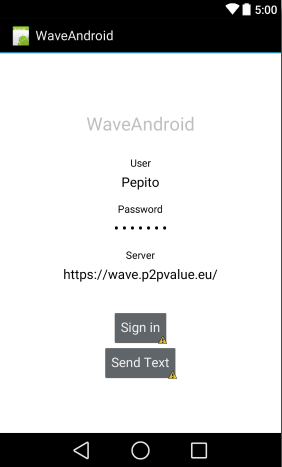
\includegraphics[keepaspectratio, scale=0.6]{Media/Captures/waveAndroidLogin.png}
      \caption{Pantalla de Login de WaveAndroid}
      \label{fig:android_waveLogin}
    \end{figure}
    
        Además decidimos mejorar el sistema de mensajes de Log de la aplicación sustituyendo el framework de la librería SLF4J para Java usada por SwellRT por una versión más reciente desarrollada para Android\cite{ref:slf4j_android}.
        
    Por último instalamos la aplicación en el emulador o el dispositivo móvil y probamos que se nos muestra la pantalla de login anterior. Introducimos los datos del servidor WIAB (en este caso utilizaremos el servidor de P2PValue desplegado para pruebas en https://wave.p2pvalue.eu/), de usuario y contraseña; y comprobamos que hemos conseguido el objetivo de esta parte del proyecto: \textbf{el login del cliente Android contra el servidor WIAB se realiza de forma correcta y sin fallos.} 
     
  \subsection{Organización y Resultados}

	Una vez conseguida la conexión al servidor desde Android, decidimos revisar el código para intentar optimizarlo y organizarlo de manera que aproveche mejor las características de Android. Además el API que permite gestionar el modelo de datos de SwellRT (Ver Sección \ref{sssec:swellRT} está escrito en java, por lo que es plenamente funcional y compatible con el código de nuestra migración a Android.  En los siguientes puntos hablaremos de dicha reorganización de código y del resultado final de esta parte del proyecto.
   
    \subsubsection{Servicio Android}
    
    NO TERMINADO
    
	Como ya se ha comentado anteriormente, el proceso de login se debe hacer en un hilo de ejecución separado del hilo principal o de UX, ya que Android no recomienda\cite{ref:android_processes} que tareas que tarden mucho tiempo en ejecutarse (cómo por ejemplo descarga de datos de la red) se ejecuten en el mismo hilo que la interfaz de usuario, pudiendo bloquear dicho hilo y obstaculizando por tanto la interacción del usuario con el dispositivo.
	
	Hasta ahora habíamos utilizado para ello una Actividad que cotenía el AsyncTask\cite{ref:android:asynctask} encargado de ejecutar el código de conexión al servidor en un hilo separado del UI Thread. Sin embargo, tal y como está definida la arquitectura de Wave y de SwellRT, la utilización de callbacks (ver secciones \ref{sssec:conHttp} y \ref{sssec:conWave}) es necesaria para notificar al resto de la aplicación de los eventos relacionados con el intercambio de datos con el servidor. Un AsyncTask ejecuta de una sola vez y de forma asíncrona el código que se le asigne a su método doInBackground(), de manera que en nuestro caso no podríamos utilizar los callbacks PORQUE... 

Además cada vez que quisiéramos realizar algún tipo de interacción con el servidor habría que utilizar un AsyncTask específico para ello, lo cual no hace sino añadir más código a la aplicación. Otra desventaja de los AsyncTask en la implementación actual es que si la Actividad que lo esta ejecutando pasa a segundo plano (por ejemplo si el usuario cambia de aplicación) se detiene el proceso de conexión. 

Considerando todo esto decidimos utilizar otro componente de Android pensado para ejecutar tareas en background y con la opción de hacerlo de forma independiente de la aplicación: el Servicio\cite{ref:android_service}.

	Un Servicio Android se diferencia de una Actividad en que es un componente que se ejecuta en segundo plano y no proporciona una interfaz de usuario con la que éste pueda interactuar. Un Servicio ejecuta tareas de larga duración (cómo la descarga de datos de la red) a petición de otros componentes de la aplicación que estén "suscritos" (el término utilizado por android es "bind") a dicho Servicio, a modo de cliente-servidor. De esta manera la Actividad (cliente) que se suscriba al Servicio (servidor) puede interactuar con éste último haciendo peticiones y recibiendo notificaciones cuando el Servicio obtenga resultados. Pero un Servicio se ejecuta dentro del mismo proceso que el UI Thread, por lo que aun así tendremos que utilizar 
	
	WebSocket usa AsyncTask?
	HANDLER -> MENSAJES
    CIERRE DE APLICACIÓN
    
    
    \subsubsection{Resultado de la Migración}
    
    Después de todos estos pasos disponíamos de una versión funcional de SwellRT capaz de conectarse al servidor WIAB de forma nativa desde Android. \textbf{El resultado de esto se puede ver en el GitHub de esta parte del proyecto}\cite{ref:wave_migration_github}.
    
    Solo restaba poner el API de SwellRT encima de lo nuestro para poder acceder y trabajar a nivel de wave con el modelo de datos de SwellRT. De esto se encargó uno de los desarrolladores del proyecto inicial, Pablo Ojanguren, con el cual habiamos trabajado para realizar lo anteriormente descrito.
    
    El API con el cliente de SwellRT adaptado a Android, con el cual trabajaremos en la siguiente parte del proyecto para crear una aplicación Android que haga uso de ella, se encuentra en el GitHub de SwellRT\cite{ref:swellRT_android_github}. 
    
    
    \subsubsection{Diagramas y Dependencias}
    
    	El cliente Android de SwellRT migrado y desarrollado en esta parte del proyecto hace uso de las siguientes dependencias con librerías externas a Android:
    	
    	
    	TABLA 
    	\begin{table}[h]
  \footnotesize
  \begin{center}
    \begin{tabular}{ | c | c | p{5cm} | }
      \hline
      \textbf{Nombre} & \textbf{Versión} & \textbf{Descripción}\\
      \hline
      WAsync\cite{ref:wAsync_github} & 1.4.3 & WebSockets/HTTP Client Library for Asynchronous Communication \\
      \hline
      AsyncHttpClient \cite{ref:asyncHttpClient} & 1.8.14 & Library that allows Java applications to easily execute HTTP requests and asynchronously process the HTTP responses. \\
      \hline
      Grizzly \cite{ref:grizzly} & 2.3.18 \\
      \hline
      \hline
    \end{tabular}
  \end{center}
  \caption{Technologies Summary}
  \label{fig:technologies}
\end{table}
    	
    	